\chapter{Architektura}

\section{Markitektura 4+1}

\subsection{Diagram architektury}

\begin{figure}[h!]
    \centering
    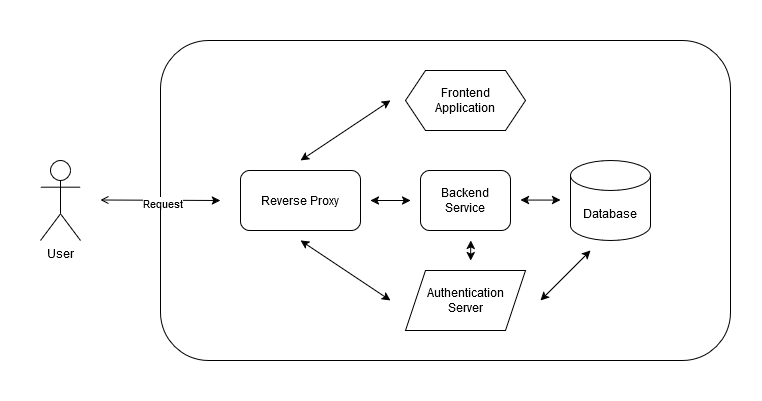
\includegraphics[width=0.99\textwidth]{resources/local/diagram-architektury.png}
    \caption{Diagram architektury}
\end{figure}

\subsection{Perspektywa logiczna}

\subsubsection*{Scenario manager}
Moduł globalny jest centralnym elementem systemu, odpowiedzialnym za zarządzanie scenariuszami użytkownika. \\

\textbf{Główne funkcje:}
\begin{itemize}
    \item Punkt wejściowy do widoku szczegółowego.
    \item Przedstawienie oraz umożliwienie zarządzania scenariuszami użytkownika.
\end{itemize}

\textbf{Kluczowe elementy:}
\begin{table}[H]
    \centering
    \begin{tabular}{|l|p{10cm}|}
        \hline
        \textbf{Element} & \textbf{Opis} \\
        \hline
        Lista scenariuszy & Zawiera scenariusze, do których użytkownik posiada uprawnienia. \\
        \hline
    \end{tabular}
\end{table}

\vspace{1em}

\subsubsection*{Object catalogue}
Moduł przeznaczony dla typów asocjacji oraz szablonów i typów obiektów.

\textbf{Główne funkcje:}
\begin{itemize}
    \item Przedstawienie oraz umożliwienie zarządzania danymi globalnymi.
\end{itemize}

\textbf{Kluczowe elementy:}
\begin{table}[H]
    \centering
    \begin{tabular}{|l|p{10cm}|}
        \hline
        \textbf{Element} & \textbf{Opis} \\
        \hline
        Lista szablonów obiektów & Przechowuje informacje o wszystkich szablonach obiektów. \\
        \hline
        Lista typów obiektów & Przechowuje informacje o wszystkich typach obiektów. \\
        \hline
        Lista typów asocjacji & Przechowuje informacje o wszystkich typach asocjacji. \\
        \hline
    \end{tabular}
\end{table}

\vspace{1em}

\subsubsection*{Timeline}
Moduł przeznaczony do wizualizacji scenariusza.

\textbf{Główne funkcje:}
\begin{itemize}
    \item Ukazanie faz oraz wątków scenariusza w czasie.
    \item Ukazanie zmian obiektów w poszczególnych momentach.
\end{itemize}

\textbf{Kluczowe elementy:}
\begin{table}[H]
    \centering
    \begin{tabular}{|l|p{10cm}|}
        \hline
        \textbf{Element} & \textbf{Opis} \\
        \hline
        Oś czasu & Ukazuje relacje pomiędzy wątkami oraz fazy scenariusza. \\
        \hline
        Widok szczegółowy wydarzenia & Ukazuje zmiany asocjacji oraz atrybutów obiektów. \\
        \hline
    \end{tabular}
\end{table}

\subsection{Perspektywa procesu}

Proces wysłania żądania przez istniejącego użytkownika systemu:

\textbf{Krok 1:} Klient wysyła żądanie HTTP/HTTPS do bramy wejściowej systemu, którą jest Reverse proxy. 

\textbf{Krok 2:} Reverse Proxy przekazuje żądanie do Authentication Server. 

\textbf{Krok 3:} Jeżeli dane autoryzacji są poprawne generowany oraz zwracany jest token JWT służący do autoryzacji. 

\textbf{Krok 4:} Wykonywane jest żądanie na konkretny endpoint Backend Service, wraz z wcześniej uzyskanym tokenem.

\textbf{Krok 5:} Żądanie jest realizowane poprzez kolejne warstwy aplikacji, skuktując zwróceniem statusu sukcesu lub błędu. 
W scenariuszu sukcesu, aplikacja najpewniej zrealizowała zmiany w Database lub zwróciła z niej dane.


\subsection{Perspektywa fizyczna}

System aktualnie nie funkcjonuje na żadnej infrastrukturze fizycznej lub chmurowej. Aczkolwiek, komponenty oraz ich zależności
zdefiniowane są za pomocą dockera, co w prosty sposób umożliwia uruchomienie systemu na środowisku produkcyjny lub w środowisku
deweloperskim (lokalnym), używanego w celu dalszego rozwoju projektu.

\subsection{Perspektywa implementacyjna}

\begin{itemize} 
    \item \textbf{Reverse Proxy} - Serwer proxy, jest bramą do systemu, która obsługuje ruch przychodzący i kieruje żądania HTTP/HTTPS do odpowiednich usług. W naszej architekturze rolę tę pełni \textbf{NGINX}.
    \item \textbf{Frontend Application} - Aplikacja webowa udostępniająca graficzny interfejs użytkownika (UI), stworzona przy użyciu frameworka React i języka TypeScript. Serwuje statyczne pliki (HTML, CSS, JS) i komunikuje się z backendem za pomocą API.
    \item \textbf{Backend Service} - Aplikacja stworzona za pomocą frameworka \textbf{Spring Boot} oraz języka Java, realizująca logikę biznesową, poprzez odpowiednie przetwarzanie żądań API oraz komunikację z bazą danych i serwerem uwierzytelniania.
    \item \textbf{Authentication Server} - Serwer uwierzytelniania i autoryzacji \textbf{Keycloak}. To popularne narzędzie umożliwia zarządzanie tożsamościami użytkowników zgodne z najnowszyszymi standardami.
    \item \textbf{Database} - Relacyjna baza danych \textbf{PostgreSQL}, przechowująca dane aplikacji.
\end{itemize}

\section{Decyzje architektoniczne}

\begin{table}[H]
    \centering
    \begin{tabular}{|p{4cm}|p{10cm}|}
        \hline
        \textbf{Decyzja} & \textbf{Opis} \\
        \hline
        Architektura klient-serwer & Jest to odpowiedni wybór dla naszych wymagań, ponieważ architektura ta 
        zakłada jasny podział ról: frontend (klient), backend (serwer), jest prosta do skalowania oraz umożliwia centralizację danych.  \\
        \hline
        Obsługa zapytań poprzez REST API & REST to najpopularniejsze rozwiązanie w architekturze klient-serwer. Bardzo dobrze pasuje
        do realizowania operacji CRUD, na ktorych opiera się nasza aplikacja. Integruje się także w prosty sposób z innymi usługami. \\
        \hline
        Websocket & Został użyty do dezauktualizowania danych, które zostały zmienione przez innego użytkownika. Umożliwia natychmiastowe
        powiadomienie frontendu o zajściu zmian w aktualnie wyświetlanym scenariuszu, poprzez analizowanie zmian w bazie danych. \\
        \hline 
        Użycie konteneryzacji &  Umożliwiło to nam uruchomienie wszystkich wymaganych komponentów systemu lokalnie w celu rozwoju aplikacji,
        oraz testowania jej działania. Konteneryzacja za pomocą Dockera ułatwi także firmie, która będzie kontynuowała projekt, dalszy
        rozwój aplikacji oraz ewentualnie uruchomienie serwisu na infrastrukturze fizycznej lub chmurowej. \\
        \hline
        Reverse Proxy jako punkt wejściowy systemu & 
        \begin{itemize}
            \setlength\itemsep{0.1em} 
            \item \textbf{Bezpieczeństwo:} ukrycie wewnętrznej struktury systemu oraz blokowanie podejrzanych adresów IP i ataków DDoS.
            \item \textbf{Wydajność:} równoważenie obciążenia oraz caching.
            \item \textbf{Skalowalność:} ułatwia wdrażanie systemu na etap produkcyjny.
        \end{itemize} \\
        \hline
        Keycloak zamiast własnego rozwiązania & Pozwoliło nam to na wprowadzenie mechanizmu 
        uwierzytelniania oraz autoryzacji zgodnego z najnoszymi standardami przy małym nakładzie czasu. System ten jest bardzo 
        elastyczny oraz skalowalny co ułatwi dalszy rozwój aplikacji. Udostępnia także użyteczny panel administartora, który w dostępny sposób
        umożliwia zarządzanie użytkownikami oraz konfiguracją. \\
        \hline
        Relacyjna baza danych & Dane w naszym systemie są strukturalne i wymagają relacji. Poszczególne obiekty w bazie danych wymagają
        jasno zdefiniowanych atrybutów. Wymagana jest także transakcyjność, dzięki czemu operacje są niezawodne, spójne oraz odtwarzalne.  \\
        \hline
    \end{tabular}
    \caption{Podjęte decyzje architektoniczne}
\end{table}

\section{Wykorzystane technologie}
W naszym projekcie wykorzystaliśmy następujące technologie:
\begin{description}
    \item[Java 21] Jest to obiektowy, wydajny i uniwersalny język programowania. Wybrany przez nas ze względu na to, że każdy z nas ma w nim doświadczenie, jest to jeden z najpopularniejszych języków programowania, posiada rozbudowane zaplecze bibliotek, a także jest łatwy w implementacji.
    \item[Spring Boot] Jest to framework używany do implementacji mechanizmów REST API, zawiera wiele bibliotek, które ułatwiają pracę nad projektem. Został przez nas wybrany ze względu na bardzo dobre działanie z językiem programowania Java 21.
    \item[PostgreSQL] Jest to system, który został stworzony w celu utrzymywania relacyjnych baz danych. Wybraliśmy go ze względu na wysoką wydajność, oraz dobrą integrację z naszym projektem.
    \item[Docker Compose] Używany przez nas w celu konteneryzacji, co zapewnia łatwe wdrożenie i odpalanie aplikacji w różnych środowiskach.
    \item[Nginx] Jest to oprogramownie działające jako serwer proxy.
    \item[TypeScript] Język programownia używany na frontendzie. Wybrany ze względu na łatwość implementacji oraz kontroli nad komponentami.
    \item[HTML i CSS] Podstawowe języki umożliwiające tworzenie struktury oraz stylizację aplikacji.
    \item[React] Jest to biblitoka, dostarczająca dynamiczne rozwiązania na frontendzie, łatwe tworzenie komponentów oraz dobrą integrację z API.
    \item[JUnit] Biblioteka używana do implementacji testów jednostkowych. Wybrana ze względu na perfekcyjną kompatybilność z Java 21.
    \item[Git] System kontrolii wersji oprogramowania. Zapewnia wysoką wydajność pracy zespołu.
    \item[Github] Platforma, która umożliwia zdalne utrzymywanie repozytorium projektu.
    \item[Github Issues] Używane jako miejsce, w którym zespół przypisywał oraz dzielił się zadaniami podczas sprintów.
    \item[Swagger] Narzędzie umożliwiające tworzenie dokumentacji API. Wybrane ze względu na kompatybilność z wcześniejszymi technologiami takimi jak Java 21 oraz Spring Boot oraz przez doświadczenie zespołu w tej technologii.
    \item[Postman] Oprogramowanie do testowania interfejsu API. Używana do bieżącego sprawdzania poprawności danych zapytań.
    \item[Husky] Narzędzie, które umożliwia lintowanie kodu lub sprawdzanie poprawności kodu przed commitem.
    \item[Intellij IDEA] Jest to środowisko programistyczne stworzone w celu tworzenia aplikacji w języku Java. Wybrane przez nas głównie ze względu na wszechstronność.
\end{description}

\section{Logika biznesowa}

\subsection{Dodawanie scenariusza}

\subsubsection{Cel operacji}
Utworzenie nowego scenariusza, który służy jako główny kontener organizujący wydarzenia, wątki i obiekty w określonych ramach czasowych.

\subsubsection{Operacja}
Proces dodawania scenariusza obejmuje:
\begin{enumerate}
    \item \textbf{Konfigurację podstawową}
    \begin{itemize}
        \item Określenie ram czasowych (data początku i końca).
        \item Zdefiniowanie jednostki czasu dla wydarzeń.
        \item Ustalenie metadanych (tytuł, opis, kontekst, cel).
    \end{itemize}
    \item \textbf{Inicjalizację struktury}
    \begin{itemize}
        \item Utworzenie wątku globalnego do zarządzania głównymi wydarzeniami.
        \item Przygotowanie dostępnych typów obiektów w scenariuszu.
    \end{itemize}
    \item \textbf{Konfigurację uprawnień}
    \begin{itemize}
        \item Przypisanie twórcy jako właściciela scenariusza.
        \item Nadanie pełnych uprawnień administracyjnych.
    \end{itemize}
\end{enumerate}

\subsubsection{Ograniczenia biznesowe}
\begin{itemize}
    \item Ramy czasowe muszą być logicznie spójne (data końcowa później niż początkowa).
    \item Każdy scenariusz musi mieć dokładnie jednego właściciela.
    \item Scenariusz musi posiadać wątek globalny do synchronizacji wydarzeń.
\end{itemize}

\subsubsection{Rezultat}
Utworzony scenariusz wraz z możliwymi do wykorzystania podstawowymi typami i zdefiniowanym wątkiem globalnym.

\subsection{Usuwanie scenariusza}

\subsubsection{Cel}
Usunięcie scenariusza wraz z zawartymi w nim wydarzeniami, wątkami i obiektami.

\subsubsection{Operacja}
Proces usuwania scenariusza obejmuje:
\begin{enumerate}
    \item \textbf{Usuwanie obiektów}
    \begin{itemize}
        \item Wraz z nimi usuwane są wszelkie ich zmiany.
    \end{itemize}
    \item \textbf{Usuwanie wątków}
    \begin{itemize}
        \item Usuwanie rozgałęzień.
        \item Usuwanie wydarzeń.
    \end{itemize}
    \item \textbf{Usuwanie samego scenariusza}
    \begin{itemize}
        \item Wraz z nim pozostałych powiązań.
    \end{itemize}
\end{enumerate}

\subsubsection{Ograniczenia biznesowe}
Usuwający musi być autorem scenariusza.

\subsubsection{Rezultat}
Usunięty scenariusz wraz z wszystkimi śladami jego obecności.

\subsection{Aktualizacja metadanych scenariusza}

\subsubsection{Cel}
Zmiana kontekstu scenariusza.

\subsubsection{Operacja}
Proces zmiany kontekstu scenariusza obejmuje wprowadzenie i zapisanie zmienionych informacji.

\subsubsection{Ograniczenia biznesowe}
Wprowadzone dane muszą istnieć (nie można wprowadzić wartości \texttt{null}).

\subsubsection{Rezultat}
Zmienione metadane scenariusza.

\subsection{Dodawanie wątku}

\subsubsection{Cel}
Dodanie nowego wątku w scenariuszu.

\subsubsection{Operacja}
Wątek może być dodany na dwa różne sposoby (nie uwzględniając wątku globalnego wstawianego automatycznie wraz z tworzeniem scenariusza). Istnieją trzy podstawowe sposoby dodania wątku - jeden bezpośredni i dwa pośrednie. 
Sposób bezpośredni obejmuje zwykłe wstawienie wątku w określonym czasie, natomiast pośrednie wstawienie rozgałęzień.
\begin{itemize}
    \item W przypadku "zwykłego" wątku obiekty możliwe są do dodania ręcznie.
    \item W przypadku łączenia wątków (\texttt{JOIN}) wszystkie obiekty z wątków wchodzących przekazywane są do nowego wątku.
    \item W przypadku podziału wątku należy zdefiniować, które obiekty mają być przekazane do którego potomka.
\end{itemize}

\paragraph{Bezpośredni} Proces wstawienia takiego wątku obejmuje:
\begin{enumerate}
    \item \textbf{Konfigurację podstawową}
    \begin{itemize}
        \item Zdefiniowanie podstawowych danych oraz czasu powstania wątku (konkretna akcja).
    \end{itemize}
    \item \textbf{Inicjalizację odpowiednich struktur}
    \begin{itemize}
        \item Dodanie wątku skutkuje wstawieniem wydarzeń \texttt{START} na jego początek oraz \texttt{END} na bezpośrednio kolejną akcję.
    \end{itemize}
\end{enumerate}

\paragraph{Pośredni}
Dodanie rozgałęzienia \texttt{JOIN} skutkuje utworzeniem jednego nowego wątku z połączenia innych, a \texttt{FORK} stworzeniem wielu wątków z jednego.

\subsubsection{Ograniczenia biznesowe}
W przypadku dodawania wątku bezpośrednio brak, dla rozgałęzień opisany oddzielnie.

\subsubsection{Rezultat}
Utworzenie nowego wątku.

\subsection{Zmiana informacji wątku}

\subsubsection{Cel}
Zmiana informacji określonych w wątku.

\subsubsection{Operacja}
Operacja obejmuje wprowadzenie zmienionych danych i ich zapisanie.

\subsubsection{Ograniczenia biznesowe}
Nie można wstawić pustych danych.

\subsubsection{Rezultat}
Zmiana danych wątku.

\subsection{Usuwanie wątku}

\subsubsection{Cel}
Usunięcie danego wątku.

\subsubsection{Operacja}
Ze względu na możliwe powiązania z innymi wątkami jest to operacja dość niebezpieczna, gdyż usuwa także wszystkie wątki bezpośrednio wynikające z usuwanego. 
\begin{enumerate}
    \item \textbf{Analizę wątków}
    \begin{itemize}
        \item Znajdowane są wszystkie wątki bezpośrednio wynikające z danego wątku za pomocą rozgałęzień.
        \item \texttt{FORK} w całości zależy od konkretnego wątku.
        \item \texttt{JOIN} tylko jeżeli wszystkie wątki wchodzące do niego zależą od jednego wątku.
        \item W przypadku pozostawienia jednego wątku wchodzącego do łączenia nie jest ono potrzebne i w dalszej części będzie usunięte.
    \end{itemize}
    \item \textbf{Usunięcie danych wątków}
    \begin{itemize}
        \item Usuwany jest dany wątek i wszystkie z niego wynikające.
        \item Usuwane są niepotrzebne rozgałęzienia.
    \end{itemize}
    \item \textbf{Usunięcie łączeń jeden-do-jednego}
    \begin{itemize}
        \item Wszystkie znalezione rozgałęzienia są usuwane.
        \item Wydarzenia wątku wychodzącego są przenoszone do wątku wchodzącego, który jest odpowiednio wydłużany.
    \end{itemize}
\end{enumerate}

\subsubsection{Ograniczenia biznesowe}
Brak.

\subsubsection{Rezultat}
Usunięcie wątku wraz z wszystkimi innymi, które były od niego zależne.

\newpage
\section{Schemat bazy danych}

\begin{figure}[h!]
    \centering
    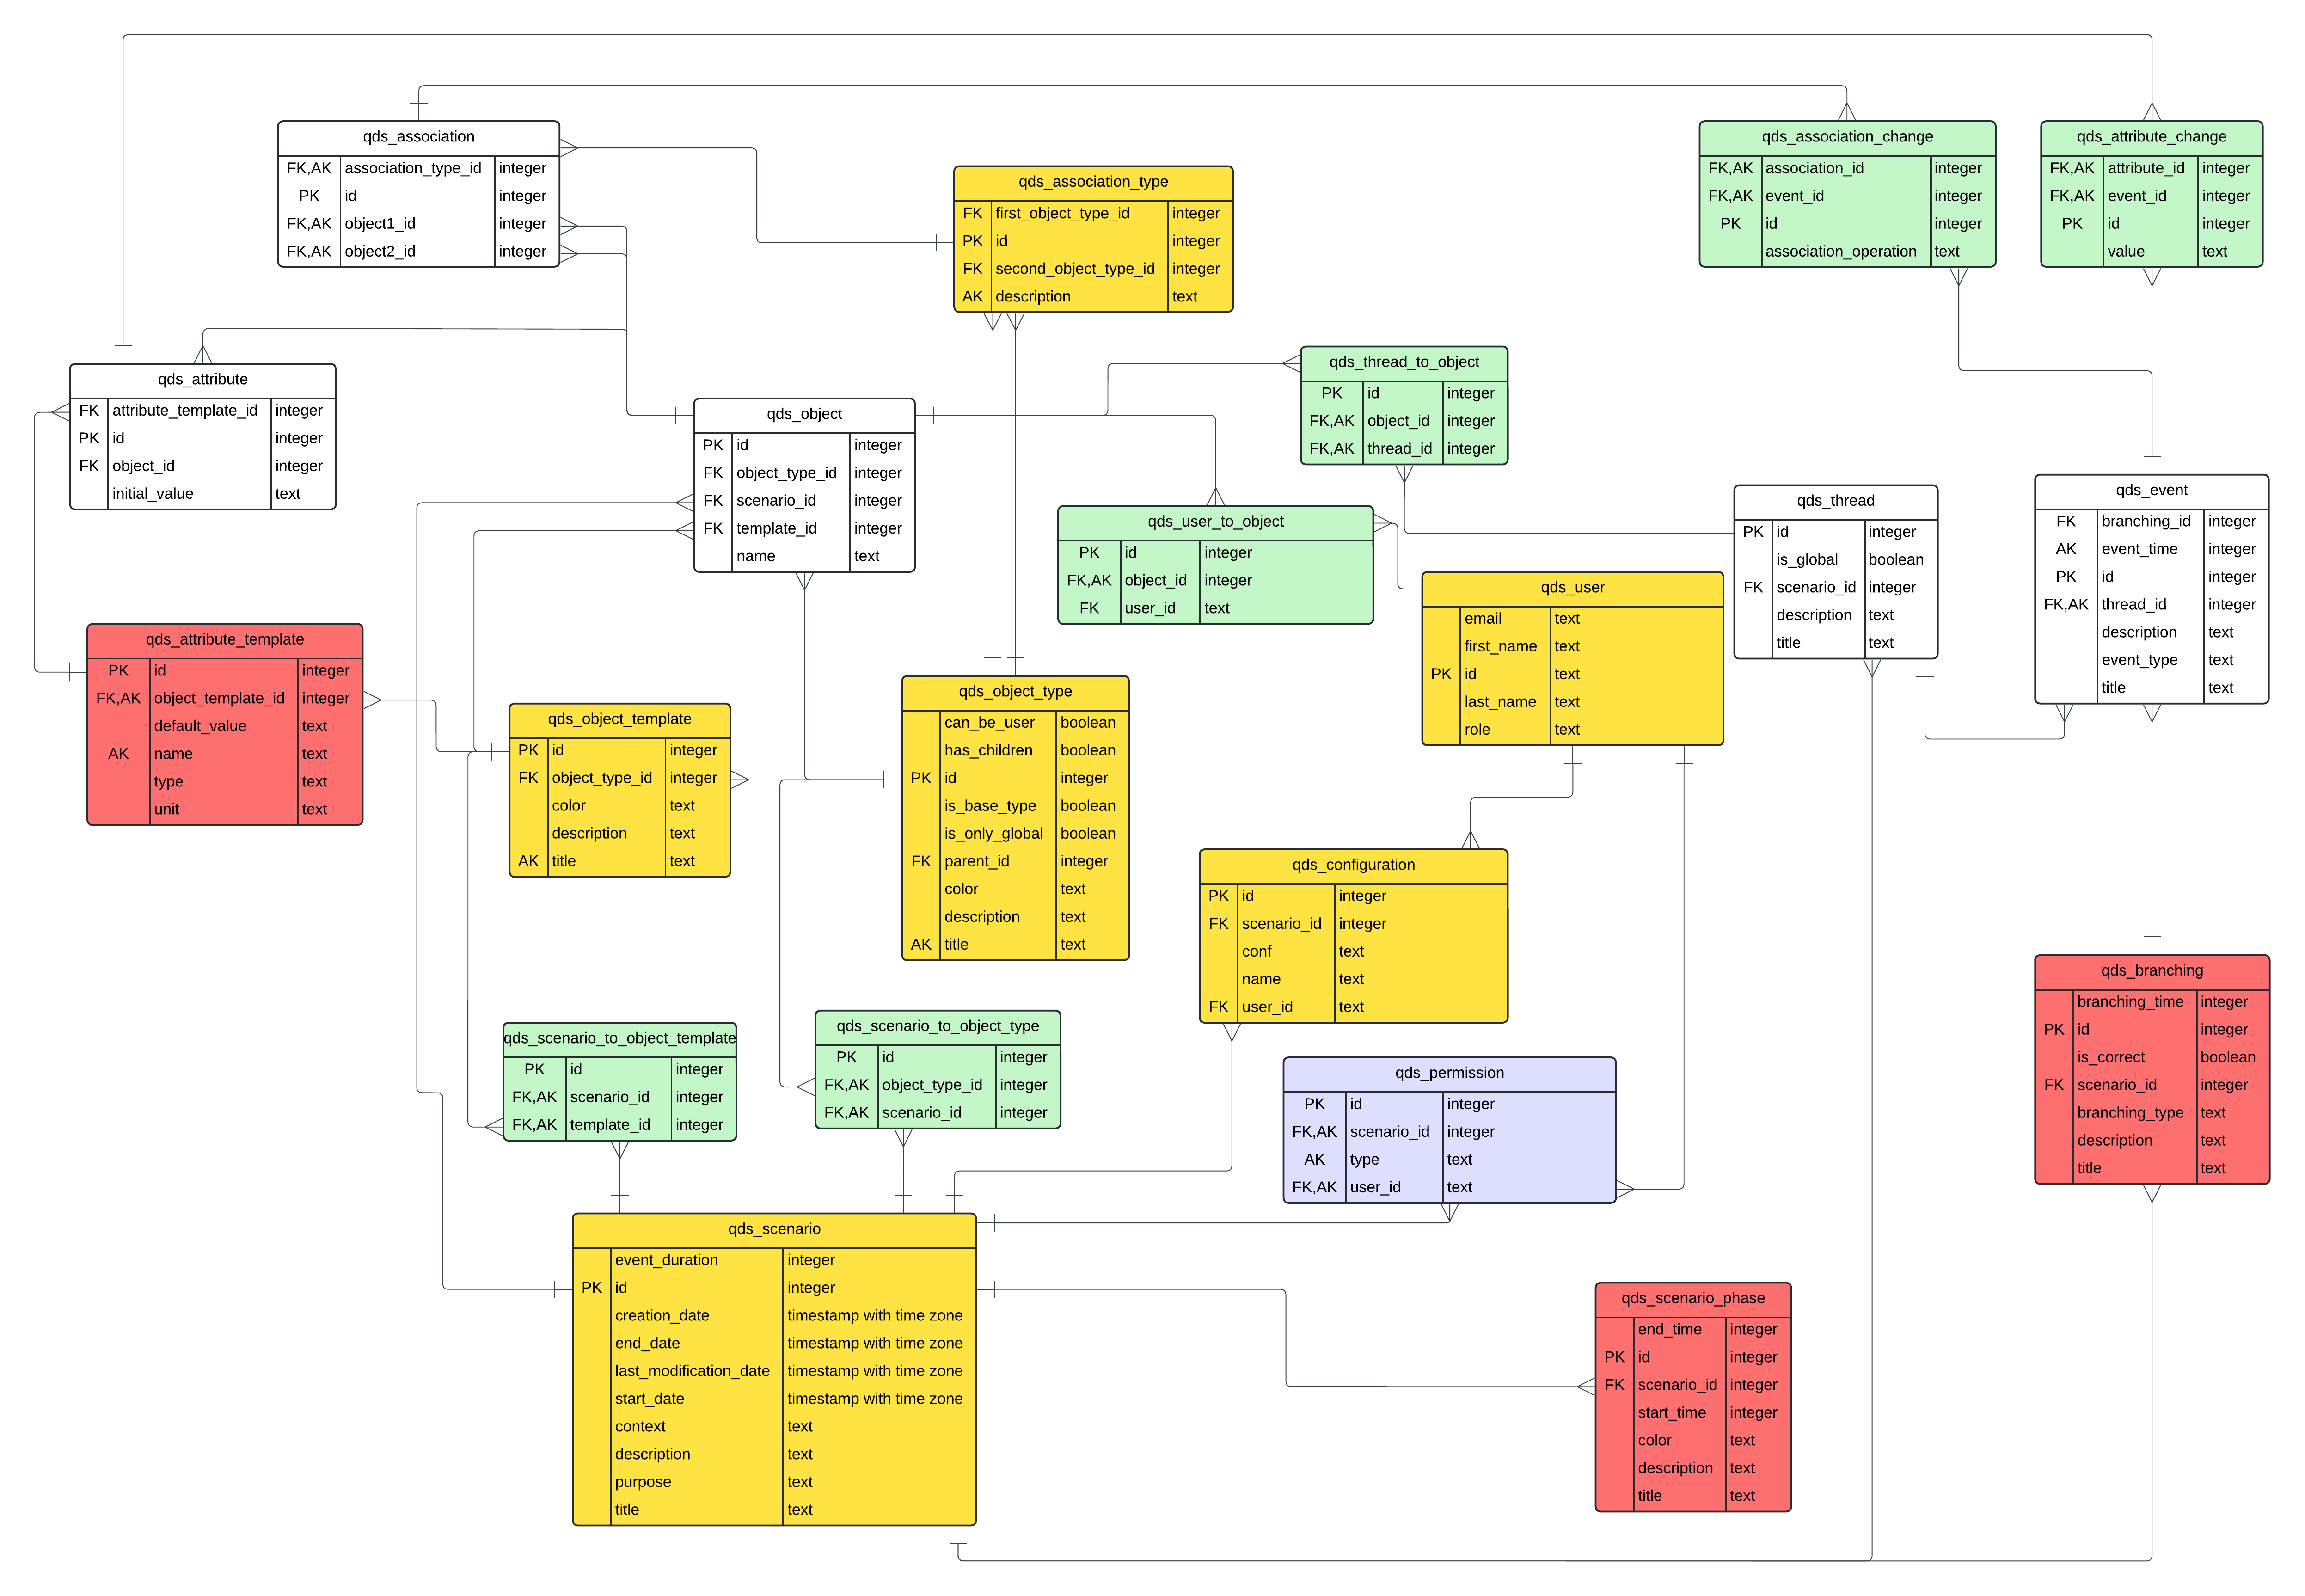
\includegraphics[width=0.99\textwidth]{resources/local/baza-danych-schemat.png}
    \caption{Schemat bazy danych}
\end{figure}

Legenda kolorów:
\begin{itemize}
    \item Żółte - encje globalne współdzielone pomiędzy scenariuszami.
    \item Zielone - encje realizujące relacje wiele do wielu.
    \item Białe - główne encje, które są wyłączne dla każdego scenariusza.
    \item Czerwone - encje pomocnicze.
    \item Niebieski - encje definiujące uprawnienia.
\end{itemize}

\section{Opis encji}

\subsection{Encje scenariuszowe}

\begin{figure}[H]
    \begin{minipage}{\textwidth}
        \centering

        \begin{figure}[H]
            \centering
            \begin{minipage}{0.8\textwidth}
                \begin{framed}
                    \noindent\textbf{\large Nazwa techniczna:} \texttt{qds\_scenario} \\
                    \textbf{\large Nazwa robocza:} Scenariusz \\
                    \textbf{\large Opis:} Reprezentuje scenariusz, centralny element systemu organizujący
                    wydarzenia, wątki i obiekty w określonych ramach czasowych.
                \end{framed}
            \end{minipage}
        \end{figure}


        \begin{table}[H]
            \centering
            \renewcommand{\arraystretch}{1.6}
            \begin{tabular}{|>{\bfseries}l|p{0.7\textwidth}|}
                \hline
                \rowcolor[HTML]{EFEFEF} \textbf{Atrybut} & \textbf{Opis} \\
                \hline
                \texttt{id} & Unikalny identyfikator scenariusza. \\
                \hline
                \texttt{title} & Nazwa scenariusza. \\
                \hline
                \texttt{description} & Opis scenariusza mający przybliżyć najważniejsze informacje na jego temat. \\
                \hline
                \texttt{context} & Kontekst w jakim ma miejsce scenariusz. \\
                \hline
                \texttt{purpose} & Cel przewodni scenariusza. \\
                \hline
                \texttt{event\_duration} & Domyślny czas trwania zdarzenia, wyrażony za pomocą wewnętrznej dla scenariusz jednostki czasu. \\
                \hline
                \texttt{start\_date} & Dokładny moment w czasie rozpoczęcia scenariusza, uwzględniający strefę czasową. \\
                \hline
                \texttt{end\_date} & Dokładny moment w czasie zakończenia scenariusza, uwzględniający strefę czasową. \\
                \hline
                \texttt{creation\_date} & Dokładny moment w czasie utworzenia scenariusza, uwzględniający strefę czasową. \\
                \hline
                \texttt{last\_modification\_date} & Dokładny moment w czasie ostatniej aktualizacji scenariusza, uwzględniający strefę czasową. \\
                \hline
            \end{tabular}
            \caption{Atrybuty encji \texttt{scenariusza}}
        \end{table}
    \end{minipage}
\end{figure}

\begin{figure}[H]
    \begin{minipage}{\textwidth}
        \centering
        \begin{figure}[H]
            \centering
            \begin{minipage}{0.8\textwidth}
                \begin{framed}
                    \noindent\textbf{\large Nazwa techniczna:} \texttt{qds\_scenario\_phase} \\
                    \textbf{\large Nazwa robocza:} Faza scenariusza \\
                    \textbf{\large Opis:} Reprezentuje logiczną fazę czasową w scenariuszu.
                    Fazy pozwalają na podział scenariusza na mniejsze, znaczące okresy, ułatwiając organizację i wizualizację wydarzeń.
                \end{framed}
            \end{minipage}
        \end{figure}

        \begin{table}[H]
            \centering
            \renewcommand{\arraystretch}{1.6}
            \begin{tabular}{|>{\bfseries}l|p{0.8\textwidth}|}
                \hline
                \rowcolor[HTML]{EFEFEF} \textbf{Atrybut} & \textbf{Opis} \\
                \hline
                \texttt{id} & Unikalny identyfikator fazy scenariusza. \\
                \hline
                \texttt{title} & Nazwa fazy scenariusza. \\
                \hline
                \texttt{description} & Opis fazy scenariusza mający przybliżyć najważniejsze informacje na jej temat. \\
                \hline
                \texttt{color} & Kolor zapisany heksadecymalnie, który zostanie użyty podczas wizualizacji fazy. \\
                \hline
                \texttt{start\_date} & Czas rozpoczęcia fazy scenariusza, wyrażony za pomocą wewnętrznej dla scenariusz jednostki czasu. \\
                \hline
                \texttt{end\_date} & Czas zakończenia fazy scenariusza, wyrażony za pomocą wewnętrznej dla scenariusz jednostki czasu. \\
                \hline
                \texttt{scenario\_id} & Klucz obcy scenariusza, do którego należy faza scenariusza. \\
                \hline
            \end{tabular}
            \caption{Atrybuty encji \texttt{fazy scenariusza}}
        \end{table}
    \end{minipage}
\end{figure}

\subsection{Encje konfiguracyjne}

\begin{figure}[H]
    \centering
    \begin{minipage}{0.8\textwidth}
        \begin{framed}
            \noindent\textbf{\large Nazwa techniczna:} \texttt{qds\_user} \\
            \textbf{\large Nazwa robocza:} Użytkownik \\
            \textbf{\large Opis:} Reprezentuje użytkownika systemu. Przechowuje podstawowe informacje o użytkowniku
            oraz jego rolę systemową.
        \end{framed}
    \end{minipage}
\end{figure}

\begin{table}[H]
    \centering
    \renewcommand{\arraystretch}{1.6}
    \begin{tabular}{|>{\bfseries}l|p{0.8\textwidth}|}
        \hline
        \rowcolor[HTML]{EFEFEF} \textbf{Atrybut} & \textbf{Opis} \\
        \hline
        \texttt{id} & Unikalny identyfikator użytkownika. \\
        \hline
        \texttt{email} & Adres e-mail użytkownika. \\
        \hline
        \texttt{first\_name} & Imię użytkownika. \\
        \hline
        \texttt{last\_name} & Nazwisko użytkownika. \\
        \hline
        \texttt{role} & Rola użytkownika:
        \begin{itemize}
            \item \texttt{USER} - Zwykły użytkownik.
            \item \texttt{ADMIN} - Administrator systemu.
        \end{itemize} \\
        \hline
    \end{tabular}
    \caption{Atrybuty encji \texttt{użytkownika}}
\end{table}

\begin{figure}[H]
    \centering
    \begin{minipage}{0.8\textwidth}
        \begin{framed}
            \noindent\textbf{\large Nazwa techniczna:} \texttt{qds\_permission} \\
            \textbf{\large Nazwa robocza:} Permisja \\
            \textbf{\large Opis:} Określa poziomy uprawnień dostępu do scenariusza.
        \end{framed}
    \end{minipage}
\end{figure}

\begin{table}[H]
    \centering
    \renewcommand{\arraystretch}{1.6}
    \begin{tabular}{|>{\bfseries}l|p{0.8\textwidth}|}
        \hline
        \rowcolor[HTML]{EFEFEF} \textbf{Atrybut} & \textbf{Opis} \\
        \hline
        \texttt{id} & Unikalny identyfikator permisji. \\
        \hline
        \texttt{role} & Typ uprawnienia:
        \begin{itemize}
            \item \texttt{AUTHOR} - Pełne uprawnienia, włącznie z zarządzaniem dostępem.
            \item \texttt{EDIT} - Możliwość modyfikacji scenariusza.
            \item \texttt{VIEW} - Podgląd scenariusza.
        \end{itemize} \\
        \hline
        \texttt{scenario\_id} & Klucz obcy scenariusza, do którego odnosi się permisja. \\
        \hline
        \texttt{user\_id} & Klucz obcy użytkownika, do którego odnosi się permisja. \\
        \hline
    \end{tabular}
    \caption{Atrybuty encji \texttt{permisji}}
\end{table}

\begin{figure}[H]
    \centering
    \begin{minipage}{0.8\textwidth}
        \begin{framed}
            \noindent\textbf{\large Nazwa techniczna:} \texttt{qds\_configuration} \\
            \textbf{\large Nazwa robocza:} Konfiguracja \\
            \textbf{\large Opis:} Przechowuje globalne ustawienia konfiguracyjne systemu. Zawiera domyślne wartości
            i parametry wpływające na działanie całego systemu.
        \end{framed}
    \end{minipage}
\end{figure}

\begin{table}[H]
    \centering
    \renewcommand{\arraystretch}{1.6}
    \begin{tabular}{|>{\bfseries}l|p{0.8\textwidth}|}
        \hline
        \rowcolor[HTML]{EFEFEF} \textbf{Atrybut} & \textbf{Opis} \\
        \hline
        \texttt{id} & Unikalny identyfikator konfiguracji. \\
        \hline
        \texttt{name} & Nazwa ustawień, unikalna dla scenariusza oraz użytkownika. \\
        \hline
        \texttt{conf} & Dane konfiguracji przechowywane w formacie JSON. \\
        \hline
        \texttt{scenario\_id} & Klucz obcy scenariusza, do którego odnosi się konfiguracja. \\
        \hline
        \texttt{user\_id} & Klucz obcy użytkownika, do którego odnosi się konfiguracja. \\
        \hline
    \end{tabular}
    \caption{Atrybuty encji \texttt{konfiguracji}}
\end{table}

\subsection{Encje Typów}

\begin{figure}[H]
    \centering
    \begin{minipage}{0.8\textwidth}
        \begin{framed}
            \noindent\textbf{\large Nazwa techniczna:} \texttt{qds\_object\_type} \\
            \textbf{\large Nazwa robocza:} Typ obiektu \\
            \textbf{\large Opis:} Definiuje typ obiektu w systemie, określając jego podstawowe właściwości
            i ograniczenia. Typy mogą tworzyć hierarchię (dziedziczenie) i definiować zasady globalności obiektów.
        \end{framed}
    \end{minipage}
\end{figure}

\begin{table}[H]
    \centering
    \renewcommand{\arraystretch}{1.6}
    \begin{tabular}{|>{\bfseries}l|p{0.8\textwidth}|}
        \hline
        \rowcolor[HTML]{EFEFEF} \textbf{Atrybut} & \textbf{Opis} \\
        \hline
        \texttt{id} & Unikalny identyfikator typu obiektu. \\
        \hline
        \texttt{title} & Unikalny tytuł typu obiektu. \\
        \hline
        \texttt{description} & Opis typu obiektu. \\
        \hline
        \texttt{color} & Kolor zapisany heksadecymalnie, który zostanie użyty podczas wizualizacji obiektu. \\
        \hline
        \texttt{is\_only\_global} & Wartość logiczna stwierdziająca czy obiekt może być tylko w wątku globalnym. \\
        \hline
        \texttt{has\_children} & Wartość logiczna stwierdziająca czy obiekt posiada potomne typy. \\
        \hline
        \texttt{is\_base\_type} & Wartość logiczna stwierdziająca czy jest typem podstawowym, tworzonym przy tworzeniu scenariusza. \\
        \hline
        \texttt{can\_be\_user} & Wartość logiczna stwierdziająca czy obiekt może być przydzielony do użytkownika. \\
        \hline
        \texttt{parent\_id} & Klucz obcy typu nadrzędnego, za pomocą którego tworzy się hierarchia. \\
        \hline
    \end{tabular}
    \caption{Atrybuty encji \texttt{typu obiektu}}
\end{table}

Dodatkowe informacje:
\begin{itemize}
    \item Nie można usunąć typu używanego przez obiekty lub szablony.
    \item Usunięcie typu jest możliwe tylko gdy nie ma typów potomnych.
\end{itemize}

\begin{figure}[H]
    \centering
    \begin{minipage}{0.8\textwidth}
        \begin{framed}
            \noindent\textbf{\large Nazwa techniczna:} \texttt{qds\_association\_type} \\
            \textbf{\large Nazwa robocza:} Typ asocjacji \\
            \textbf{\large Opis:} Definiuje typ/rodzaj asocjacji możliwy między obiektami w systemie.
            Określa jakie typy obiektów mogą być połączone danym rodzajem asocjacji.
        \end{framed}
    \end{minipage}
\end{figure}

\begin{table}[H]
    \centering
    \renewcommand{\arraystretch}{1.6}
    \begin{tabular}{|>{\bfseries}l|p{0.8\textwidth}|}
        \hline
        \rowcolor[HTML]{EFEFEF} \textbf{Atrybut} & \textbf{Opis} \\
        \hline
        \texttt{id} & Unikalny identyfikator typu asocjacji. \\
        \hline
        \texttt{description} & Opis asocjacji \\
        \hline
        \texttt{firstObjectTypeId} & Identyfikator pierwszego dozwolonego typu obiektu. \\
        \hline
        \texttt{secondObjectTypeId} & Identyfikator drugiego dozwolonego typu obiektu. \\
        \hline
    \end{tabular}
    \caption{Atrybuty encji \texttt{typu asocjacji}}
\end{table}

Dodatkowe informacje:
\begin{itemize}
    \item Nie można usunąć używanego typu asocjacji.
    \item Typ obiektu posiada relacje wiele do wielu z encją scenariusza.
\end{itemize}

\subsection{Encje szablonowe}

\begin{figure}[H]
    \centering
    \begin{minipage}{0.8\textwidth}
        \begin{framed}
            \noindent\textbf{\large Nazwa techniczna:} \texttt{qds\_object\_template} \\
            \textbf{\large Nazwa robocza:} Szablon obiektu \\
            \textbf{\large Opis:} Reprezentuje szablon obiektu określający jego strukturę atrybutów.
            Definiuje jakie atrybuty i jakiego typu musi posiadać obiekt stworzony na podstawie tego szablonu.
        \end{framed}
    \end{minipage}
\end{figure}

\begin{table}[H]
    \centering
    \renewcommand{\arraystretch}{1.6}
    \begin{tabular}{|>{\bfseries}l|p{0.8\textwidth}|}
        \hline
        \rowcolor[HTML]{EFEFEF} \textbf{Atrybut} & \textbf{Opis} \\
        \hline
        \texttt{id} & Unikalny identyfikator szablonu obiektu. \\
        \hline
        \texttt{title} & Unikalny tytuł szablonu. \\
        \hline
        \texttt{description} & Opis szablonu. \\
        \hline
        \texttt{color} & Kolor zapisany heksadecymalnie, który zostanie użyty podczas wizualizacji obiektu. \\
        \hline
        \texttt{object\_type\_id} & Klucz obcy typu obiektu, do którego można przypisać szablon. \\
        \hline
    \end{tabular}
    \caption{Atrybuty encji \texttt{szablonu obiektu}}
\end{table}

Dodatkowe informacje:
\begin{itemize}
    \item Nie można usunąć szablonu używanego przez obiekt.
    \item Szablon obiektu posiada relacje wiele do wielu z encją scenariusza.
\end{itemize}

\begin{figure}[H]
    \centering
    \begin{minipage}{0.8\textwidth}
        \begin{framed}
            \noindent\textbf{\large Nazwa techniczna:} \texttt{qds\_attribute\_template} \\
            \textbf{\large Nazwa robocza:} Szablon atrybutu obiektu. \\
            \textbf{\large Opis:} Reprezentuje szablon obiektu określający jego strukturę atrybutów.
            Definiuje jakie atrybuty i jakiego typu musi posiadać obiekt stworzony na podstawie tego szablonu.
        \end{framed}
    \end{minipage}
\end{figure}

\begin{table}[H]
    \centering
    \renewcommand{\arraystretch}{1.6}
    \begin{tabular}{|>{\bfseries}l|p{0.8\textwidth}|}
        \hline
        \rowcolor[HTML]{EFEFEF} \textbf{Atrybut} & \textbf{Opis} \\
        \hline
        \texttt{id} & Unikalny identyfikator szablonu obiektu. \\
        \hline
        \texttt{name} & Unikalna nazwa atrybutu. \\
        \hline
        \texttt{default\_value} & Wartość domyślna atrybutu. \\
        \hline
        \texttt{unit} & Jednostka wartości atrybutu. \\
        \hline
        \texttt{role} & Typ wartości atrybutu:
        \begin{itemize}
            \item \texttt{INT} - liczba całkowita.
            \item \texttt{STRING} - łańcuch znaków.
            \item \texttt{DATE} - data lub czas.
            \item \texttt{BOOL} - wartość logiczna.
        \end{itemize} \\
        \hline
        \texttt{object\_template\_id} & Klucz obcy szablonu obiektu, do którego przydzielony jest atrybut. \\
        \hline
    \end{tabular}
    \caption{Atrybuty encji \texttt{szablonu atrybutu obiektu}}
\end{table}

Dodatkowe informacje:
\begin{itemize}
    \item Usuwany kaskadowo wraz z szablonem obiektu.
\end{itemize}

\subsection{Encje dotyczące konkretnego obiektu}

\begin{figure}[H]
    \centering
    \begin{minipage}{0.8\textwidth}
        \begin{framed}
            \noindent\textbf{\large Nazwa techniczna:} \texttt{qds\_object} \\
            \textbf{\large Nazwa robocza:} Obiekt \\
            \textbf{\large Opis:} Reprezentuje obiekt w scenariuszu, który może być modyfikowany przez wydarzenia.
            Obiekt jest globalny jeśli został utworzony w wątku globalnym, w przeciwnym razie jest lokalny
            i przypisany do konkretnego wątku.
        \end{framed}
    \end{minipage}
\end{figure}

\begin{table}[H]
    \centering
    \renewcommand{\arraystretch}{1.6}
    \begin{tabular}{|>{\bfseries}l|p{0.8\textwidth}|}
        \hline
        \rowcolor[HTML]{EFEFEF} \textbf{Atrybut} & \textbf{Opis} \\
        \hline
        \texttt{id} & Unikalny identyfikator obiektu. \\
        \hline
        \texttt{name} & Unikalna nazwa obiektu. \\
        \hline
        \texttt{object\_type\_id} & Klucz obcy typu obiektu. \\
        \hline
        \texttt{template\_id} & Klucz obcy szablonu obiektu. \\
        \hline
        \texttt{scenario\_id} & Klucz obcy scenariusza obiektu. \\
        \hline
    \end{tabular}
    \caption{Atrybuty encji \texttt{obiektu}}
\end{table}

Dodatkowe informacje:
\begin{itemize}
    \item Obiekt można przypisać do użytkownika systemu.
\end{itemize}

\begin{figure}[H]
    \centering
    \begin{minipage}{0.8\textwidth}
        \begin{framed}
            \noindent\textbf{\large Nazwa techniczna:} \texttt{qds\_association} \\
            \textbf{\large Nazwa robocza:} Asocjacja \\
            \textbf{\large Opis:} Reprezentuje asocjację (relację) między dwoma obiektami w systemie.
            Przechowuje informacje o typie relacji i powiązanych obiektach.
        \end{framed}
    \end{minipage}
\end{figure}

\begin{table}[H]
    \centering
    \renewcommand{\arraystretch}{1.6}
    \begin{tabular}{|>{\bfseries}l|p{0.8\textwidth}|}
        \hline
        \rowcolor[HTML]{EFEFEF} \textbf{Atrybut} & \textbf{Opis} \\
        \hline
        \texttt{id} & Unikalny identyfikator asocjacji. \\
        \hline
        \texttt{association\_type\_id} & Klucz obcy typu asocjacji. \\
        \hline
        \texttt{object1\_id} & Klucz obcy pierwszego obiektu. \\
        \hline
        \texttt{object2\_id} & Klucz obcy drugiego obiektu. \\
        \hline
    \end{tabular}
    \caption{Atrybuty encji \texttt{asocjacji}}
\end{table}

Dodatkowe informacje:
\begin{itemize}
    \item Kombinacja (typ asocjacji, obiekt1, obiekt2) musi być unikalna.
    \item Usuwana automatycznie gdy usuwany jest którykolwiek z obiektów.
\end{itemize}

\begin{figure}[H]
    \centering
    \begin{minipage}{0.8\textwidth}
        \begin{framed}
            \noindent\textbf{\large Nazwa techniczna:} \texttt{qds\_attribute} \\
            \textbf{\large Nazwa robocza:} Atrybut \\
            \textbf{\large Opis:} Reprezentuje atrybut obiektu w systemie wraz z jego wartością początkową.
        \end{framed}
    \end{minipage}
\end{figure}

\begin{table}[H]
    \centering
    \renewcommand{\arraystretch}{1.6}
    \begin{tabular}{|>{\bfseries}l|p{0.8\textwidth}|}
        \hline
        \rowcolor[HTML]{EFEFEF} \textbf{Atrybut} & \textbf{Opis} \\
        \hline
        \texttt{id} & Unikalny identyfikator atrybutu. \\
        \hline
        \texttt{initial\_value} & Wartość początkowa atrybutu. \\
        \hline
        \texttt{object\_id} & Klucz obcy obiektu, którego dotyczy atrybut. \\
        \hline
        \texttt{attribute\_template\_id} & Klucz obcy szablonu atrybutu. \\
        \hline
    \end{tabular}
    \caption{Atrybuty encji \texttt{atrybutu obiektu}}
\end{table}

Dodatkowe informacje:
\begin{itemize}
    \item Każdy obiekt posiada dokładnie wszystkie atrybuty zdefiniowane przez typ obiektu.
    \item Usuwany kaskadowo z obiektem.
\end{itemize}

\subsection{Encje wizualizujące upływ czasu}

\begin{figure}[H]
    \centering
    \begin{minipage}{0.8\textwidth}
        \begin{framed}
            \noindent\textbf{\large Nazwa techniczna:} \texttt{qds\_thread} \\
            \textbf{\large Nazwa robocza:} Wątek \\
            \textbf{\large Opis:} Reprezentuje wątek w scenariuszu - sekwencję wydarzeń w czasie.
        \end{framed}
    \end{minipage}
\end{figure}

\begin{table}[H]
    \centering
    \renewcommand{\arraystretch}{1.6}
    \begin{tabular}{|>{\bfseries}l|p{0.8\textwidth}|}
        \hline
        \rowcolor[HTML]{EFEFEF} \textbf{Atrybut} & \textbf{Opis} \\
        \hline
        \texttt{id} & Unikalny identyfikator wątku. \\
        \hline
        \texttt{title} & Tytuł wątku. \\
        \hline
        \texttt{description} & Opis wątku. \\
        \hline
        \texttt{is\_global} & Wartość logiczna stwierdziająca czy wątek jest globalny, czy lokalny. \\
        \hline
        \texttt{scenario\_id} & Klucz obcy scenariusza. \\
        \hline
    \end{tabular}
    \caption{Atrybuty encji \texttt{wątku}}
\end{table}

\begin{figure}[H]
    \centering
    \begin{minipage}{0.8\textwidth}
        \begin{framed}
            \noindent\textbf{\large Nazwa techniczna:} \texttt{qds\_event} \\
            \textbf{\large Nazwa robocza:} Wydarzenie \\
            \textbf{\large Opis:} Reprezentuje wydarzenie w scenariuszu zachodzące w określonym czasie i wątku.
            Wydarzenia są podstawowym mechanizmem wprowadzania zmian w systemie,
            odpowiadają za modyfikacje atrybutów obiektów i ich asocjacji.
        \end{framed}
    \end{minipage}
\end{figure}

\begin{table}[H]
    \centering
    \renewcommand{\arraystretch}{1.6}
    \begin{tabular}{|>{\bfseries}l|p{0.8\textwidth}|}
        \hline
        \rowcolor[HTML]{EFEFEF} \textbf{Atrybut} & \textbf{Opis} \\
        \hline
        \texttt{id} & Unikalny identyfikator wydarzenia. \\
        \hline
        \texttt{title} & Tytuł wydarzenia. \\
        \hline
        \texttt{description} & Opis wydarzenia. \\
        \hline
        \texttt{event\_time} & czas wydarzenia, wyrażony za pomocą wewnętrznej dla scenariusz jednostki czasu. \\
        \hline
        \texttt{event\_type} & Typ wydarzenia.
        \begin{itemize}
            \item \texttt{GLOBAL} - Wydarzenie w wątku globalnym, nadpisuje zmiany z innych wątków.
            \item \texttt{NORMAL} - Standardowe wydarzenie w wątku.
            \item \texttt{START} - Początek wątku.
            \item \texttt{END} - Koniec wątku.
            \item \texttt{IDLE} - Wydarzenie puste.
            \item \texttt{JOIN\_OUT} - Początek wątku powstałego z połączenia.
            \item \texttt{JOIN\_IN} - Koniec wątku wchodzącego do połączenia.
            \item \texttt{FORK\_OUT} - Początek wątku powstałego z podziału.
            \item \texttt{FORK\_IN} - Wydarzenie w wątku przed podziałem.
        \end{itemize} \\
        \hline
        \texttt{thread\_id} & Klucz obcy wątku, w ramach którego ma miejsce wydarzenie. \\
        \hline
        \texttt{branching\_id} & Identyfikator powiązanego rozgałęzienia (tylko dla FORK/JOIN). \\
        \hline
    \end{tabular}
    \caption{Atrybuty encji \texttt{wydarzenia}}
\end{table}

\begin{figure}[H]
    \centering
    \begin{minipage}{0.8\textwidth}
        \begin{framed}
            \noindent\textbf{\large Nazwa techniczna:} \texttt{qds\_attribute\_change} \\
            \textbf{\large Nazwa robocza:} Zmiana atrybutu \\
            \textbf{\large Opis:} Reprezentuje zmianę wartości atrybutu w kontekście wydarzenia.
            Jest częścią historii zmian atrybutów, gdzie każda zmiana jest powiązana
            z konkretnym wydarzeniem (QdsEvent) określającym kiedy nastąpiła.
        \end{framed}
    \end{minipage}
\end{figure}

\begin{table}[H]
    \centering
    \renewcommand{\arraystretch}{1.6}
    \begin{tabular}{|>{\bfseries}l|p{0.8\textwidth}|}
        \hline
        \rowcolor[HTML]{EFEFEF} \textbf{Atrybut} & \textbf{Opis} \\
        \hline
        \texttt{id} & Unikalny identyfikator zmiany atrybutu. \\
        \hline
        \texttt{value} & Nowa wartość atrybutu. \\
        \hline
        \texttt{attribute\_id} & Klucz obcy atrybutu obiektu, którego wartość ulega zmianie. \\
        \hline
        \texttt{event\_id} & Klucz obcy wydarzenia, w ramach którego odbywa się zmiana atrybutu. \\
        \hline
    \end{tabular}
    \caption{Atrybuty encji \texttt{zmiany atrybutu obiektu}}
\end{table}

Dodatkowe informacje:
\begin{itemize}
    \item Każda zmiana musi być unikalna dla pary (wydarzenie, atrybut).
    \item Zmiany są usuwane kaskadowo wraz z wydarzeniem lub modyfikowanym atrybutem.
\end{itemize}

\begin{figure}[H]
    \centering
    \begin{minipage}{0.8\textwidth}
        \begin{framed}
            \noindent\textbf{\large Nazwa techniczna:} \texttt{qds\_association\_change} \\
            \textbf{\large Nazwa robocza:} Zmiana asocjacji \\
            \textbf{\large Opis:} Reprezentuje zmianę stanu asocjacji (dodanie/usunięcie) w określonym momencie czasu.
            Jest częścią historii zmian asocjacji, gdzie każda zmiana jest powiązana z konkretnym
            wydarzeniem określającym kiedy i w jakim kontekście nastąpiła.
        \end{framed}
    \end{minipage}
\end{figure}

\begin{table}[H]
    \centering
    \renewcommand{\arraystretch}{1.6}
    \begin{tabular}{|>{\bfseries}l|p{0.8\textwidth}|}
        \hline
        \rowcolor[HTML]{EFEFEF} \textbf{Atrybut} & \textbf{Opis} \\
        \hline
        \texttt{id} & Unikalny identyfikator zmiany asocjacji. \\
        \hline
        \texttt{association\_operation} & Rodzaj operacji
        \begin{itemize}
            \item \texttt{INSERT} - Dodanie nowej asocjacji między obiektami.
            \item \texttt{DELETE} - Usunięcie istniejącej asocjacji między obiektami.
        \end{itemize} \\
        \hline
        \texttt{association\_id} & Klucz obcy atrybutu obiektu, którego wartość ulega zmianie. \\
        \hline
        \texttt{event\_id} & Klucz obcy wydarzenia, w ramach którego odbywa się zmiana atrybutu. \\
        \hline
    \end{tabular}
    \caption{Atrybuty encji \texttt{zmiany asocjacji obiektu}}
\end{table}

Dodatkowe informacje:
\begin{itemize}
    \item Każda zmiana musi być unikalna dla pary (wydarzenie, asocjacja).
    \item Zmiany są usuwane kaskadowo wraz z wydarzeniem lub modyfikowaną asocjacją.
\end{itemize}

\section{Indeksy}

Indeks to struktura danych, pozwalająca na przyśpieszenie operacji odczytu w bazie danych.
Poprzez wygenerowaną strukturę danych, operacja szukania odpowiednich rekordów posiada o wiele mniejszą złożoność.
W naszym przypadku używamy indeksów HASH, ponieważ najlepiej sprawdzają się w operacjach równościowych.
Klucze są unikalne, co znacznie zmniejsza prawdopodobieństwo kolizji. Dodatkowo, kolejność
nie jest istotna w kolumnach identyfikujących.

\begin{itemize}
    \item \textbf{Tabela:} \texttt{qds\_scenario\_phase}, \textbf{Kolumna:} \texttt{scenario\_id}
    Indeks optymalizujący wyszukiwanie faz scenariusza po identyfikatorze scenariusza.

    \item \textbf{Tabela:} \texttt{qds\_association\_type}, \textbf{Kolumna:} \texttt{first\_object\_type\_id}
    Indeks przyspieszający wyszukiwanie asocjacji po pierwszym typie obiektu.

    \item \textbf{Tabela:} \texttt{qds\_association\_change}, \textbf{Kolumna:} \texttt{association\_id}
    Indeks optymalizujący wyszukiwanie zmian danej asocjacji.

    \item \textbf{Tabela:} \texttt{qds\_attribute\_change}, \textbf{Kolumna:} \texttt{event\_id}
    Indeks przyspieszający wyszukiwanie zmian atrybutów związanych z określonym wydarzeniem.

    \item \textbf{Tabela:} \texttt{qds\_object}, \textbf{Kolumna:} \texttt{scenario\_id}
    Indeks zapewniający unikalność obiektów w scenariuszu.

    \item \textbf{Tabela:} \texttt{qds\_thread}, \textbf{Kolumna:} \texttt{scenario\_id}, \textbf{Warunek:} \texttt{is\_global = TRUE}
    Unikalny indeks zapewniający, że w danym scenariuszu może istnieć tylko jeden wątek globalny.

    \item \textbf{Tabela:} \texttt{qds\_thread}, \textbf{Kolumna:} \texttt{scenario\_id}
    Indeks optymalizujący wyszukiwanie wątków scenariusza.

    \item \textbf{Tabela:} \texttt{qds\_branching}, \textbf{Kolumna:} \texttt{scenario\_id}
    Indeks przyspieszający wyszukiwanie rozgałęzień danego scenariuszu.

    \item \textbf{Tabela:} \texttt{qds\_event}, \textbf{Kolumna:} \texttt{thread\_id}
    Indeks optymalizujący wyszukiwanie wydarzeń danego wątku.
\end{itemize}
